\documentclass[12pt]{report}

\usepackage[a4paper]{geometry}
%\geometry{left=2.5cm,right=2.5cm,top=2.5cm,bottom=2.5cm, a4paper}
\usepackage[utf8]{inputenc}
\usepackage{amsmath}
\usepackage{amsthm}
\usepackage{amssymb}
\usepackage{ulem}
\usepackage{graphicx}
\usepackage{caption}
\graphicspath{}
\usepackage[document]{ragged2e}
\usepackage{setspace}
\usepackage{tabularx}
\usepackage[slovene]{babel}
\usepackage{textcomp, gensymb}
\usepackage{siunitx}
\usepackage{pdfrender,xcolor}
\usepackage{hyperref}
\usepackage{xurl}
\usepackage{float}
\usepackage{titlesec}

\newfloat{slika}{htbp}{loc}
\floatname{slika}{Slika}

\newfloat{tabela}{htbp}{loc}
\floatname{tabela}{Tabela}

% Differential
\newcommand{\diff}{\mathrm{d}}

\title{
  
\includegraphics[width=0.4\textwidth]{fmf_logo}\\
  {\small Oddelek za fiziko} \\
  {Spektrometer}\\
  {\small Poročilo pri fizikalnem praktikumu IV}\\

}
\date{}
\author{ Kristofer Čepon Povšič \\[5 cm]
 \small  Asistentka: Jelena Vesić  \\
}


\titleformat{\chapter}[hang]{\Huge\bfseries}{\thechapter{. }}{0pt}{\Huge\bfseries}

\setlength\parindent{0pt}

\begin{document}

\setcounter{page}{2}

\maketitle

\chapter*{Uvod}

Spektroskop je priprava za merjenje spektrov, to je porazdelitev svetlobnega toka po frekvenci ali valovni dolžini. Pri vaji bom uporabljal klasični optični spektroskop na prizmo. Delovanje temelji na principu, da se svetloba v prizmi iz stekla razcepi na raznobarvne komponente. Kot detektor bom uporabljal človeško oko, ki je najbolj občutljivo za rumenozeleno svetlobo pri valovni dolžini 555nm. Proti vijolični in rdeči barvi, ki sta meji vidnega spektra, občutljivost pada. 

Poznamo dve vrsti spektrov - zvezne (žarnice) in črtaste (plini). Če pa je dovolj velika ločljivost, pa je vsak spekter zvezen. 

\chapter*{Naloga}

\begin{enumerate}
  \item Umerite kotno skalo spektroskopa s spektralnimi črtami Hg in $\text{H}_2$
  \item Izmerite valovne dolžine spektralnih črt v spektru varčne žarnice. Primerjajte spekter s tistim, izmerjenim v Hg pod točko 1
  \item Izmerite centralno valovno dolžino in ocenite spektralno širino rdeče, rumene, zelene in modre svetleče diode (LED) 
  \item Opazujte zvezni spekter volframove žarnice in oceni valovno dolžino najsvetlejšega (rumenega) dela in zapišite intervale, ki jih pokrivajo posamezne barve
  \item Opazuje absorpcijski spekter $\text{NO}_2$ tako, da cevko s plinom presevate z belo svetlobo. 
  \item Izmerite valovne dolžine črt v spektru He in Ne. 
\end{enumerate}

\begingroup
\let\clearpage\relax

\chapter*{Potrebščine}
\begin{itemize}
  \item optični spektroskop: prizma iz kremastega stekla
  \item nosilec za spektralne cevi (ampule) z visokonapetnostnim izvorom, ampule s plini Hg, He, Ne in $\text{H}_2$
  \item varčna žarnica, LED diode, volframova žarnica, cevka z $\text{NO}_2$
\end{itemize}

\chapter*{Navodilo}

Z živim srebrom in vodikom izmerim kote in preko barv umerim spektroskop. Dobljene podatke preko enačbe 

\begin{equation}\label{eq:1}
  \phi (\lambda) = A \lambda + B \sqrt{\lambda} +C
\end{equation}

Če enačbo \ref{eq:1} preoblikujemo valovno dolžino izraženo v odvisnosti od kota:

\begin{equation}
  \lambda(\phi) =\left(\frac{-B + \sqrt{B^2 + 4A(C - \phi)}}{2A}\right)^2
\end{equation}

Pomerimo tudi varčno žarnico, različne LED diode in spektra helij in neonov. 

\endgroup


\chapter*{Obdelava podatkov}

\section*{Kalibracija}

Izmerjeni in izračunani podatki za Hg: 

\begin{tabela}[H]
  \centering
  \begin{tabular}{|c|c|c|}\hline
    barva & $\phi [^{\circ}]$ & $\lambda [nm]$ \\ \hline
    2 rumeni & 45.2 & 578 \\
    zelena & 45.4 & 546 \\ 
    modrovijolična & 47.1 & 436 \\ \hline
  \end{tabular}
\end{tabela}

Izmerjeni in izračunani podatki za $\text{H}_2$: 

\begin{tabela}[H]
  \centering
  \begin{tabular}{|c|c|c|}\hline
    barva & $\phi [^{\circ}]$ & $\lambda [nm]$ \\ \hline
    rdeča & 44.5 & 656 \\
    svetlomodra & 46.0 & 486 \\ 
    modrovijolična & 47.2 & 434 \\ \hline
  \end{tabular}
\end{tabela}

Izračunamo parametre: 

\begin{align*}
  A &= 94 \pm 8 \\
  B &= 6 \cdot 10^{7} \pm 1 \cdot 10^{7} \\
  C &= -11 \cdot 10^{4} \pm 2 \cdot 10^{4}
\end{align*}

Regresiven graf pa izgleda: 

\begin{slika}[H]
  \centering
  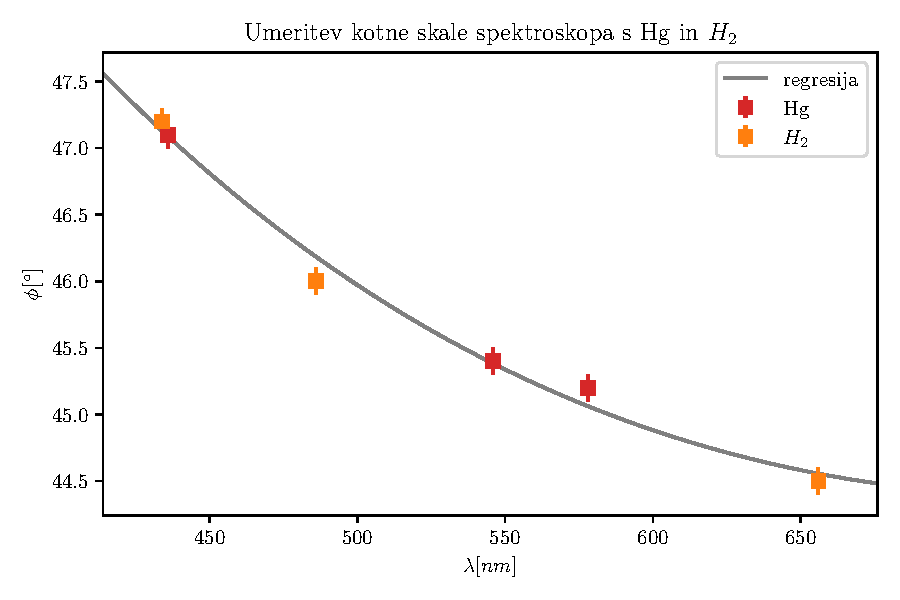
\includegraphics{kalibracija}
  \caption{\small Izmerjeni koti in izračunane valovne dolžine za živo srebro in vodik.}
\end{slika}

\section*{Varčna žarnica}

\begin{tabela}[H]
  \centering
  \begin{tabular}{|c|c|c|}\hline
    barva & $\phi [^{\circ}]$ & $\lambda [nm]$ \\ \hline
    vijolična & 47.3 &   425.8\\
    modra 1 & 46.4 &   472.9\\
    modra 2 & 45.8 &   512.2\\
    zelena 1 & 45.5 &   535.7\\
    zelena 2 &  45.2 &   563.3 \\ \hline
  \end{tabular}
\end{tabela}

\begin{slika}[H]
  \centering
  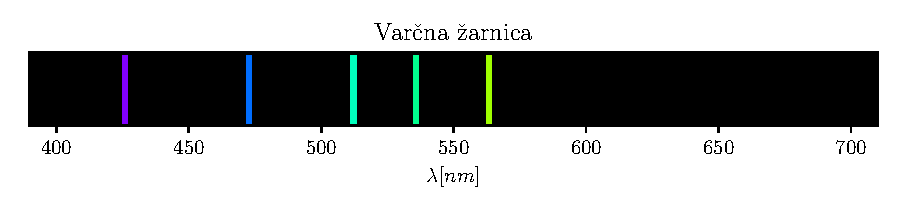
\includegraphics{Vzarnica}
  \caption{\small Spekter varčne žarnice}
\end{slika}

\section*{LED diode}

\begin{tabela}[H]
  \centering
  \begin{tabular}{|c|c|c|c|c|}\hline
    barva & $\phi_{min} [^{\circ}]$ & $\phi_{max} [^{\circ}]$ & $\lambda_{min} [nm]$ & $\lambda_{max} [nm] $\\ \hline
    modra & 47.1 &    46.0 &   435.4 &   498.1\\
    rumena & 45.4 &    45.1 &   544.4 &   573.8\\
    rdeča & 45.0 &    44.7 &   585.2 &   627.3\\
    zelena & 45.6 &    45.0 &   527.5 &   585.2\\ \hline 
  \end{tabular}
\end{tabela}

\begin{slika}[H]
  \centering
  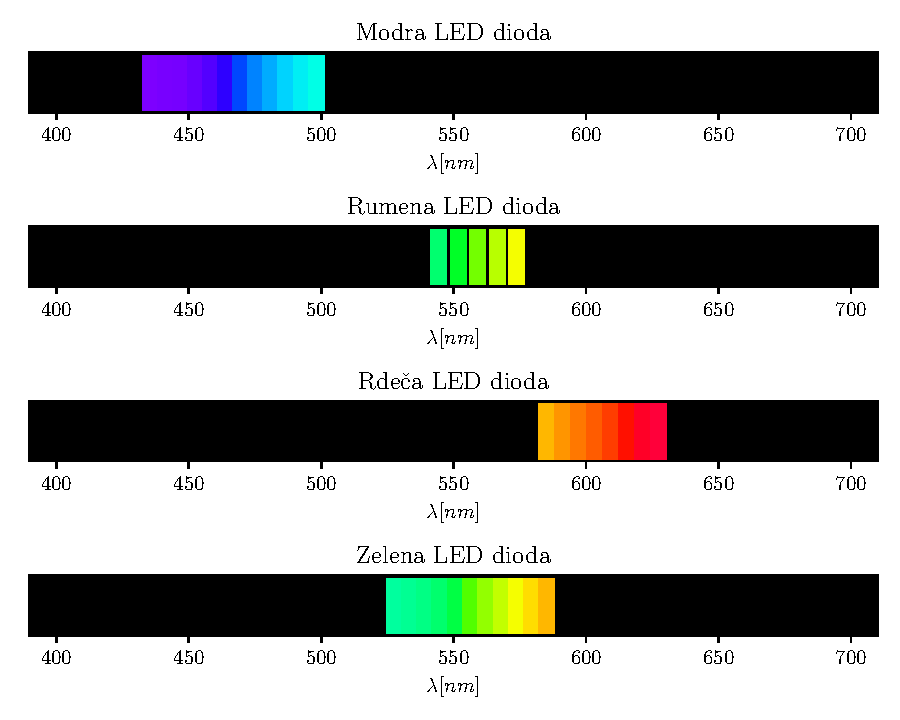
\includegraphics{led}
  \caption{\small Spekter LED diode}
\end{slika}

\section*{Volfram žarnica}

\begin{slika}[H]
  \centering
  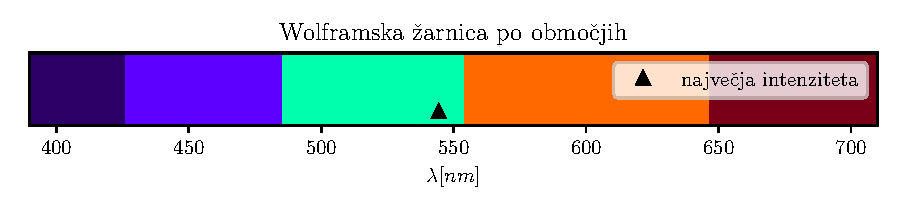
\includegraphics{wolfram}
  \caption{\small Spekter volfram žarnice z valovno dolžine največje jakosti - ocenjene s prostim očesom.}
\end{slika}

\section*{Absorpcijski spekter $\text{NO}_2$}

\begin{tabela}[H]
  \centering
  \begin{tabular}{|c|c|}\hline
    $\phi [^{\circ}]$ & $\lambda [nm]$ \\ \hline
    45.1 &   573.8\\
    45.3 &   553.6\\
    45.5 &   535.7\\
    45.8 &   512.2\\
    46.1 &   491.5\\
    46.3 &   478.9\\
    46.5 &   467.0\\
    46.7 &   455.9\\
    46.7 &   455.9 \\ \hline
  \end{tabular}
\end{tabela}

\begin{slika}[H]
  \centering
  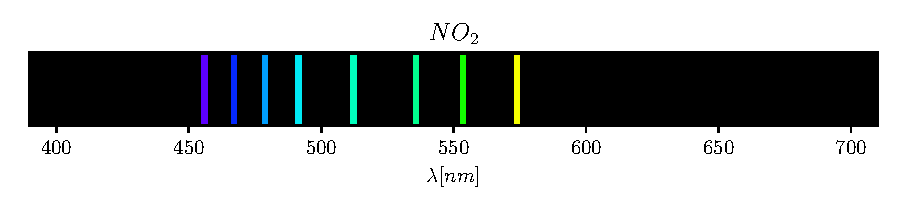
\includegraphics{no2}
  \caption{\small Absorpcijski spekter $\text{NO}_2$}
\end{slika}

\section*{He in Ne}

Izmerjene vrednosti helija: 

\begin{tabela}[H]
  \centering
  \begin{tabular}{|c|c|}\hline
    $\phi [^{\circ}]$ & $\lambda [nm]$ \\ \hline
    44.5 &   670.3\\
    44.6 &   646.1\\
    45.1 &   573.8\\
    45.9 &   505.0\\
    46.0 &   498.1\\
    46.4 &   472.9\\
    46.8 &   450.6\\
    47.0 &   440.3 \\ \hline
  \end{tabular}
\end{tabela}

\begin{slika}[H]
  \centering
  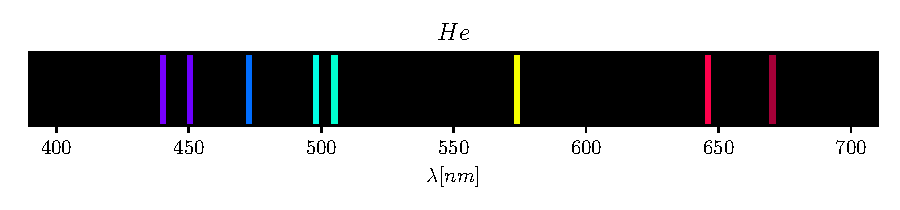
\includegraphics{He}
  \caption{\small Spekter helija.}
\end{slika}

Izmerjene vrednosti neona: 

\begin{tabela}[H]
  \centering
  \begin{tabular}{|c|c|}\hline
    $\phi [^{\circ}]$ & $\lambda [nm]$ \\ \hline
    45.0 &   585.2\\
    45.2 &   563.3\\
    45.4 &   544.4\\
    45.8 &   512.2\\
    46.7 &   455.9\\ \hline
  \end{tabular}
\end{tabela}

\begin{slika}[H]
  \centering
  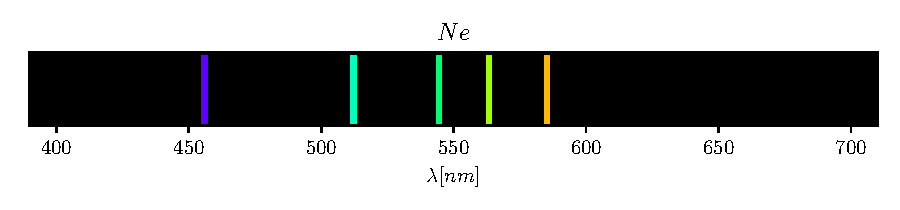
\includegraphics{Ne}
  \caption{\small Spekter neona}
\end{slika}


\end{document}
